\documentclass[a4paper, 10pt]{scrartcl}
\usepackage[a4paper,top=2.9cm,bottom=2.9cm,left=2.7cm,right=2.7cm]{geometry}
\usepackage[utf8]{inputenc}
% PACCHETTO PER LA LINGUA
\usepackage[english]{babel}
% PACCHETTI PER EQUAZIONI E SIMBOLI MATEMATICI
\usepackage{amsmath}
\usepackage{amsfonts}
\usepackage{amssymb}
\usepackage{mathabx}
\usepackage{mathtools}
%\usepackage{cancel}
% PACCHETTI PER FIGURE, SUBFIGURE E FIGURE PLACEMENT
%\usepackage{wrapfig}
\usepackage{subcaption}
\usepackage{sidecap}
\sidecaptionvpos{figure}{t}
\usepackage{float}
% PACCHETTI PER CAPTION E TABELLE
\usepackage{caption}
\captionsetup{tableposition=bottom, figureposition=bottom, font=small}
\captionsetup[subfigure]{width=0.9\textwidth, format=hang}

% PACCHETTI PER GRAFICA E COLORI
\usepackage{graphicx}
\usepackage[dvipsnames]{xcolor}

% RIFERIMENTI IPERTESTUALI
\usepackage[colorlinks, citecolor=NavyBlue, linkcolor=blue, unicode]{hyperref}
%% autoref di equazioni con (numero)
\addto\extrasenglish{\def\equationautorefname~#1\null{(#1)\null}}
% PACCHETTI VARI E PERSONALIZZAZIONI
%\usepackage{mparhack}
%\usepackage{ragged2e}

% PACCHETTO PER BIBLIOGRAFIA
%\usepackage{natbib}
%\bibliographystyle{unsrt}
\usepackage[sorting=none]{biblatex}
\usepackage{csquotes}
\addbibresource{citations.bib}
\DeclareSourcemap{
  \maps[datatype=bibtex]{
    \map{
      % Remove language
      \step[fieldset=language, null]
    }
    \map{
      % If it contains a field eprinttype...
      \step[fieldsource=eprinttype, final]
      % ... remove the urldate and url
      \step[fieldset=urldate, null]
      \step[fieldset=url, null]
    }
    \map{
      % If it is not @online, always remove urldate and url
      \pernottype{online}
      % ... remove the urldate and url
      \step[fieldset=urldate, null]
      \step[fieldset=url, null]
    }
    \map{
      % If it is @online remove month, year, urldate
      \pertype{online}
      \step[fieldset=urldate, null]
      \step[fieldset=month, null]
      \step[fieldset=year, null]
    }
  }
}

\setlength\parindent{0pt}

\title{\LARGE{Report of second year activities}}
\author{\large{PhD student: Dario Zarcone}\\\large{Supervisor: Prof. Salvatore Miccichè}}
\date{\normalsize{October 20th, 2025}}
\subject{\small{Università degli Studi di Palermo\\Dipartimento di Fisica e Chimica - Emilio Segrè\\PhD Course in Physical and Chemical Sciences\\Cycle XXXIX}}

\begin{document}
\maketitle

This report summarizes the activities and projects I undertook during the second year of my PhD in Physical Sciences at the University of Palermo. My work, continuing from the first year, focused on two main topics: the application of complex systems methods on a dataset of homicides in Sicily, and the development of tools for processing text documents at scale.

The former involved a collaboration with the Prosecutor's Office of Palermo, who provided the dataset and valuable insights into the context of the data; the latter involved a collaboration with the Institute for Cross-Disciplinary Physics and Complex Systems (IFISC) in Palma de Mallorca, Spain, where I spent a four months visiting period under the supervision of Prof. David Sanchez to learn advanced text analysis techniques on a newspaper dataset.

I also worked on the development of change point analysis techniques, focusing on methods for detecting changes in time series, with applications in both the homicide dataset and the newspaper corpus.

The following sections detail these projects, concluding with a list of conferences I attended and publications I contributed to during this year.

\section{Analysis of Murders in Sicily: a Point Process Perspective}

In collaboration with the Prosecutor's Office of Palermo, last year I started working on a project that focused on the study of data concerning murders, attempted murders and disappearances in Sicily. We were able to build a dataset of about 5000 events, spanning from 1945 to 2025, with information about the victim and the date of the event; in about 70\% of the cases, we also have information about the location of the event.

This dataset is particularly valuable, as the events can be considered a proxy for the activity of Mafia in Sicily. Last year I was able to perform a preliminary analysis of the data, focusing on the temporal and spatial distribution of the events. The analysis showed that, from a temporal perspective, the data shows a bursty pattern, with clusters of events occurring in short time frames followed by periods of relative calm, in a dynamics that is reminiscent of earthquake occurrences.

This year I focused on modeling the phenomenon as a \textbf{point process} in time. This approach is common in seismology, where earthquakes are modeled as points in time and space (ETAS model), in finance, in neuroscience, and was used also in the analysis of crime data \cite{mohlerSelfExcitingPointProcess2011,bacryHawkesProcessesFinance2015,laubElementsHawkesProcesses2021}.

Formally, a point process $\{T_i\}_{i \in \mathbb{N}}$ is a random collection of points on a measurable space, typically $\mathbb{R}$ for temporal processes. The \textit{arrival times} $T_i$ can be independent of each other, as in a Poisson process, or they can exhibit dependencies, as in a \textbf{self-exciting process} or \textbf{Hawkes process}. This latter case is particularly interesting, as it captures the phenomenon where the occurrence of an event increases the likelihood of subsequent events in the near future, leading to clustering behavior similar to what we observed in the data.

In a point process, it is common to define the \textbf{conditional intensity function} $\lambda(t | \mathcal{H}_t)$, which represents the instantaneous rate of occurrence of events at time $t$, given the history $\mathcal{H}_t$ of the process up to time $t$. For a Hawkes process, the conditional intensity function can be expressed as:
\begin{equation}
  \lambda(t | \mathcal{H}_t) = \mu + \sum_{T_i < t} g(t - T_i)
\end{equation}
where $\mu$ is the baseline intensity (the rate of events in the absence of self-excitation), and $g(t - T_i)$ is a triggering function that quantifies the influence of past events $T_i$ on the current intensity. A common choice for the triggering function is an exponential decay function:
\begin{equation}
  g(t - T_i) = \alpha e^{-\beta (t - T_i)}
\end{equation}
where $\alpha > 0$ controls the magnitude of the influence and $\beta > 0$ controls the decay rate. In this formulation the expected number of events triggered by a single event, known as \textbf{branching ratio}, is given by $\frac{\alpha}{\beta}$.

Given some observed data it's possible to \textit{infer} the parameters of the model: the most common frameworks are \textit{Maximum Likelihood Estimation} (MLE), \textit{Moment Matching}, \textit{Expectation-Maximization} (EM), and \textit{Bayesian Inference} \cite{laubElementsHawkesProcesses2021}.

In the case of the murders dataset the arrival times are known with only daily resolution: this kind of lack of information is called \textbf{interval censoring} \cite{laubElementsHawkesProcesses2021} in the point process literature, and it poses challenges for parameter estimation, as the actual arrival times are not observed, and a simple Maximum Likelihood Estimation (MLE) approach cannot be directly applied.

Many approaches can be used to address this issue, such as data augmentation techniques, where the unobserved arrival times are treated as latent variables and estimated alongside the model parameters using EM \cite{shlomovichParameterEstimationMethod2022} or Bayesian methods \cite{derektuckerHandlingMissingData2019}. A simpler approach is given by using a moment matching method that accounts for the censoring in the data \cite{laubElementsHawkesProcesses2021} or by jittering the arrival times within their known intervals.

By applying this latter approach on the most intense period (events from 1975 to 2000), I was able to fit the simple exponential univariate Hawkes model to the data. The branching ratio is about 0.4, indicating a significant level of self-excitation in the data. The goodness of fit can be evaluated by the CCDF of the inter-event times and by looking at the QQ-plot of the transformed inter-event times \cite{laubElementsHawkesProcesses2021}, as in \autoref{fig:hawkes-ccdf} and \autoref{fig:hawkes-qq}.

\begin{figure}[H]
    \centering
    \begin{subfigure}[t]{.49\textwidth}
        \centering
        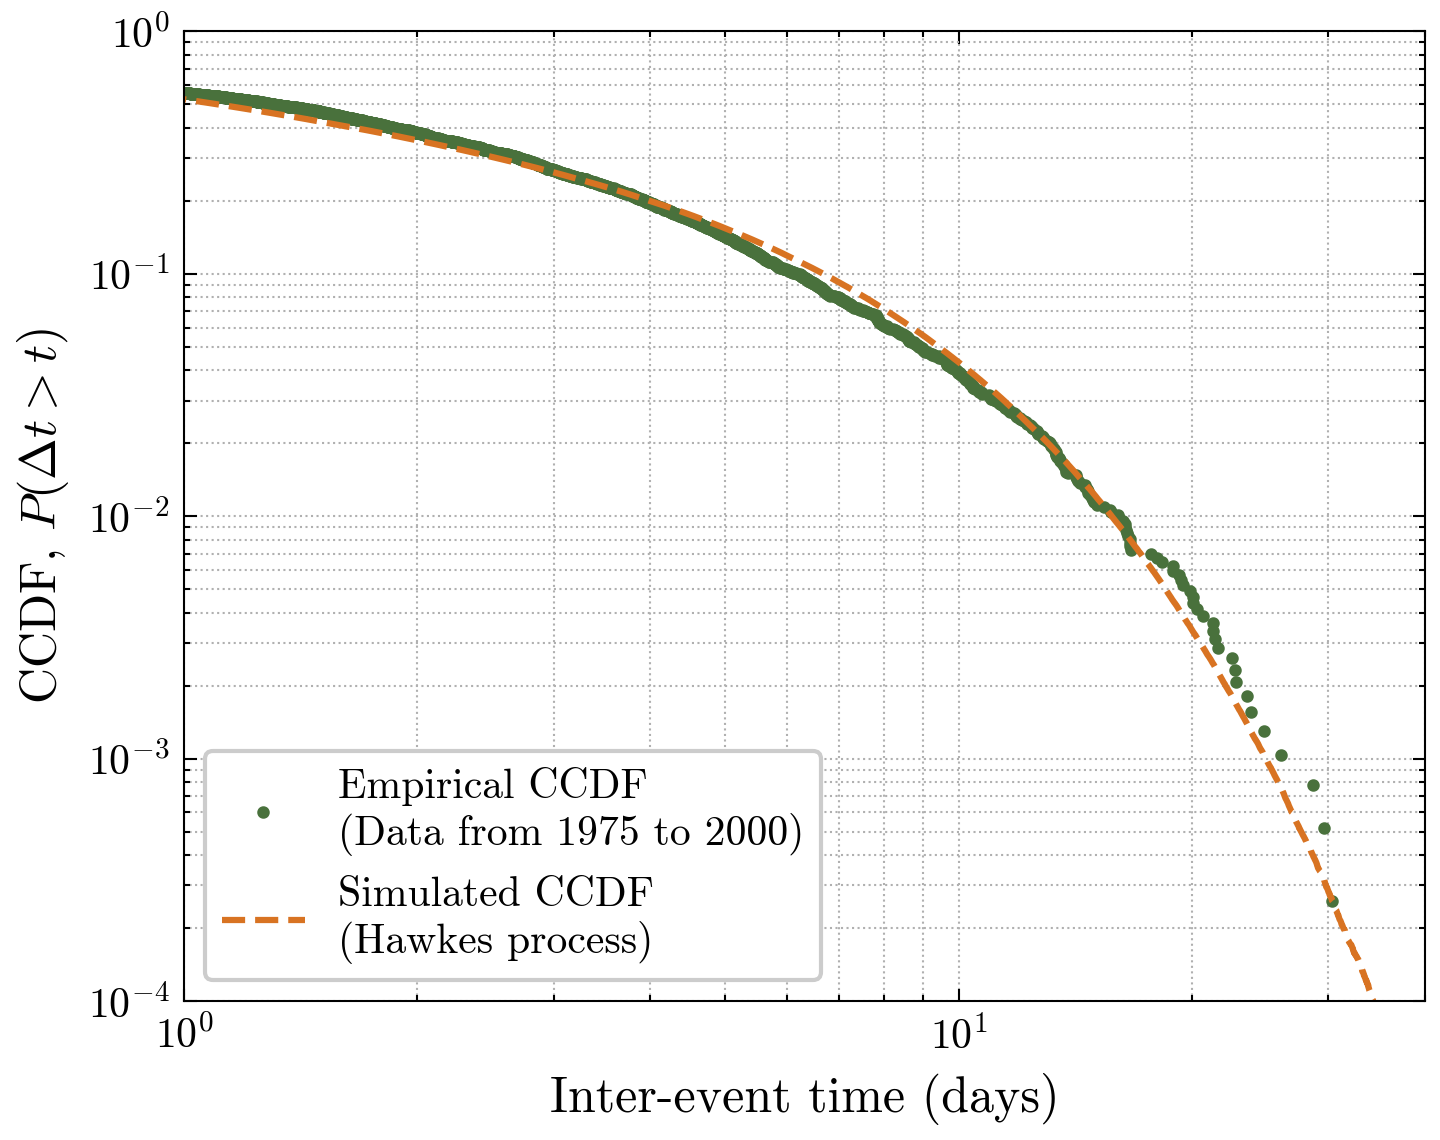
\includegraphics[width=\textwidth]{figures/hawkes-ccdf.png}
        \caption{CCDF of inter-event times in log-log scale}
        \label{fig:hawkes-ccdf}
    \end{subfigure}%
    \hspace{1em}
    \begin{subfigure}[t]{.47\textwidth}
        \centering
        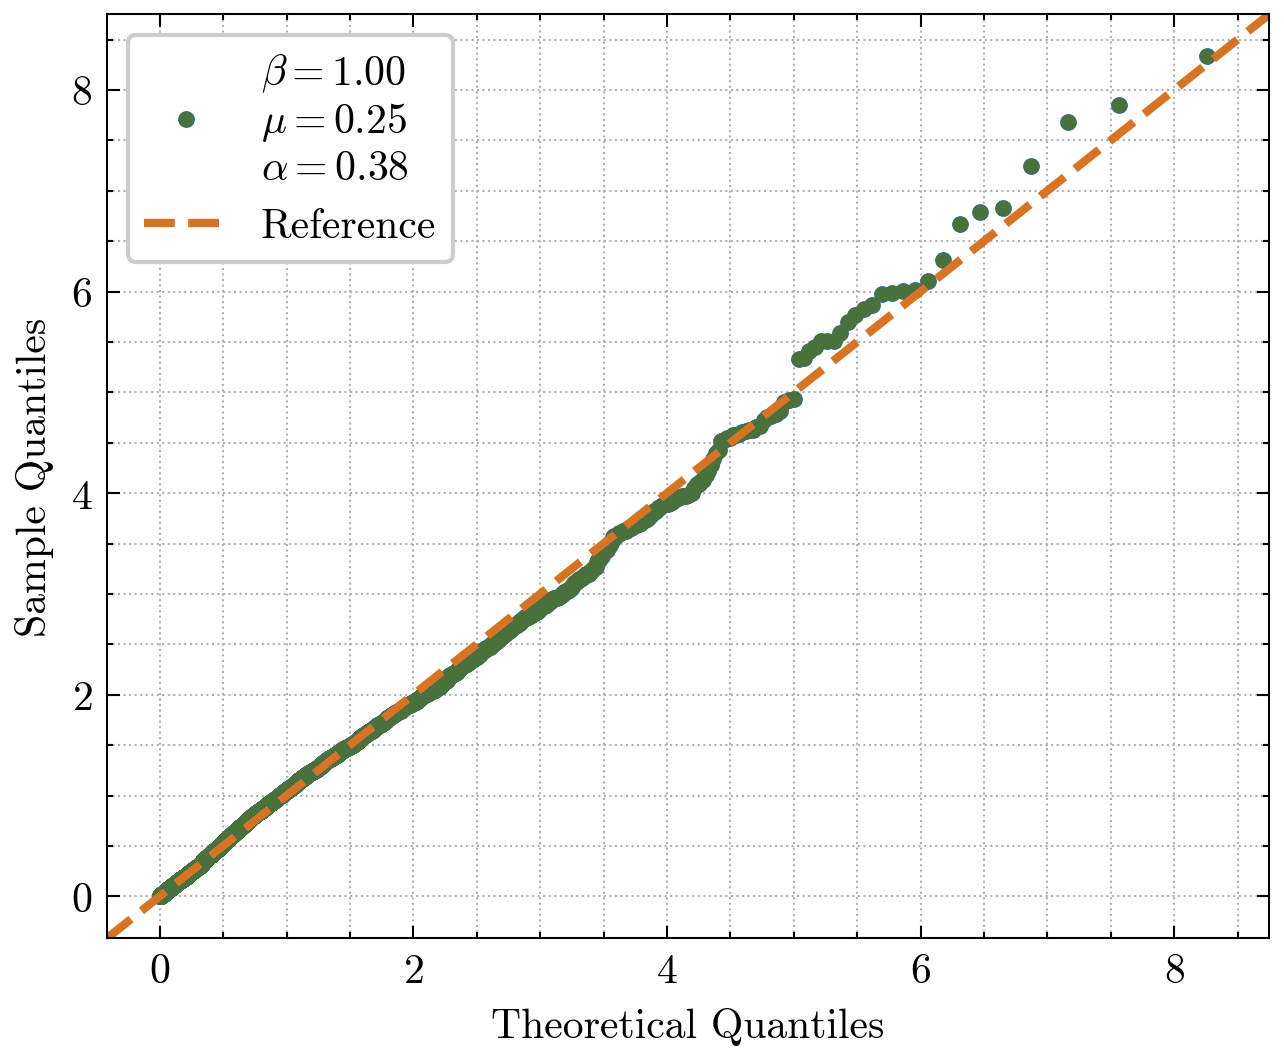
\includegraphics[width=\textwidth]{figures/hawkes-qq.png}
        \caption{QQ plot of inter-event times transformed via time-rescaling theorem with the fitted Hawkes model}
        \label{fig:hawkes-qq}
    \end{subfigure}
    \caption{Simulated vs empirical inter-event times for the fitted Hawkes model on murders in Sicily (1975-2000). The good agreement indicates a good fit of the model to the data.}
\end{figure}

The good fit of this simple model suggests that the process is self-exciting in nature: the occurrence of a murder increase the likelihood of a subsequent murder, for example because of retaliation. The model is a valid starting point for more complex analyses with different functional forms for the triggering function, incorporating also the spatial information.


\section{Text Analysis and Natural Language Processing: A Diachronic Newspaper Corpus}

Most of the data in the field of crime analysis is unstructured text data, such as police reports and court documents. Last year I focused on the development of a search engine for this kind of documents, facilitating information retrieval for the Prosecutor's Office of Palermo, that is now in use in their daily activities.

However, as the access of most of these documents is restricted, this year I focused on the corpus of all the \textbf{newspaper articles} published by \textit{La Repubblica} between 1985 and 2000, that I built by reverse engineering the CD-ROMs published by the newspaper in the early 2000s.

The dataset is formed by about \textbf{600,000} full-text articles, with metadata like the title, the date of the publication and the author. The corpus was further augmented by scraping the online archive of \textit{La Repubblica} for the section labels for more than 80\% of the articles. It's a particulary interesting set of documents, as it's very generalist and covers one of the most interesting periods in Italian history: the years of the Mafia wars, the fall of Soviet Union, the Tangentopoli corruption scandal and the beginning of the so-called \textit{Second Republic}.

Most of the analysis on the corpus was done during my visiting period at the \textit{Institute for Cross-Disciplinary Physics and Complex Systems} (IFISC) in Palma de Mallorca, Spain, where I worked from March to July 2025 under the supervision of Prof. David Sanchez.

I carried out two main projects: on one side I focused on building a \textit{topic model}, trying to understand which metodologies are best suited to \textit{label} the documents in a unsupervised way. On the other side, I used the diachronic nature of the corpus to analyze the lexical and semantic evolution over time.

From a practical standpoint, the first thing to do is preprocessing and cleaning, which involves splitting the text in words (\textit{tokenization}), removing stop words, and normalizing the text (e.g., lowercasing, stemming, lemmatization). After this step the text is converted into a vector representation, which can be sparse and word-count based (the \textit{TF-IDF} representation, which is a document-term matrix which captures the importance of words in each document) or dense and context-based (using \textit{embeddings}). A dimensionality reduction step is often applied, usually via \textit{PCA} or \textit{UMAP}. The result is a set of vectors in a lower-dimensional space that can be used for further analysis. In the case of topic modeling, clustering algorithms like \textit{K-Means} and \textit{HDBSCAN} group together similar documents.

One of the most interesting results came from the dynamical analysis: by splitting the documents by month I was able to build \textit{time series} of words importance (using TF-IDF scores) and of "\textit{media discourse}" (the center of mass of the document vectors in each month). The former can be seen as a \textit{lexical} analysis, while the latter is more \textit{semantic} in nature.

More specifically, the media discourse is computed as
\begin{equation}
    \vec{c}\,(m) = \frac{1}{N_m} \sum_{i = 1}^{N_m} \vec{d}\,_i^{(m)}
\end{equation}
where $N_m$ is the number of documents in month $m$ and $\vec{d}\,_i^{(m)}$ is the vector representation of document $i$ in month $m$. The document vectors were obtained by applying \textit{PCA} on the TF-IDF representation, keeping the first 100 components.

These time series show patterns that are consistent with the major historical changes in Italy. For example, by computing a \textit{cosine similarity matrix} (see \autoref{fig:sim_mat}) between the media discourse vectors of each month I was able to identify the Gulf War in 1991, the Kosovo War in 1999, and the beginning of the Second Republic in 1994.

%On the other hand, by estimating the Shannon entropy from the eigenvalue specrum of the covariance matrix of the documents in each month, I could identify periods of higher and lower diversity: in particular, the periods of the Gulf War and of the Kosovo War show a more focused discourse, and a lower entropy (\autoref{fig:shannon_entropy}).

\begin{SCfigure}[][ht]
    \centering
    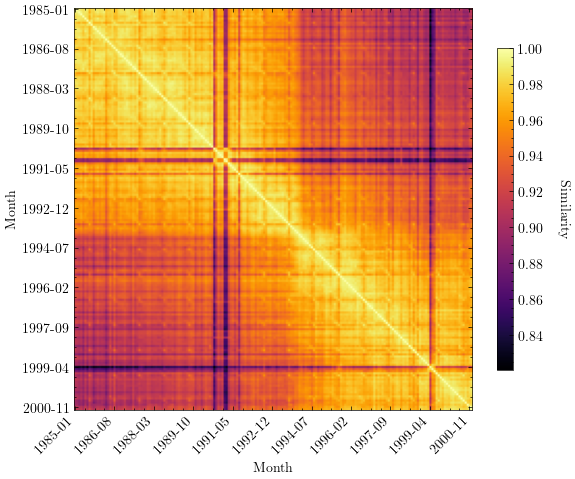
\includegraphics[width=0.5\textwidth]{figures/sim_mat.png}
    \caption{
        Cosine similarity matrix of semantic center of mass (1985-2000). 
        Darker colors indicate greater semantic change. 
        The block-diagonal structure reveals temporally coherent discourse regimes and transitions aligned with major historical events: the transition from the First to the Second Republic in 1994, the Gulf War in 1990-1991, and the Kosovo War in 1999.
    }
    \label{fig:sim_mat}
\end{SCfigure}

The techniques are very general and can be applied on other corpora, for example on the documents in the Prosecutor's Office archive. Such an approach could provide not only a useful tool for easier navigation of the documents, but also a way of defining "periods" in Mafia history based on the actual discourse, giving a quantative complement to the qualitative analysis usually done by historians and criminologists.

\section{Change Points Detection}

Both for the murders dataset and for the diachronic analysis of the newspaper corpus the time series show abrupt changes in their statistical properties. In the language of time series analysis, these points are called \textbf{change points}, and detecting them is a crucial step in understanding the underlying dynamics of the data.

Many algorithms exist for change point detection \cite{truongSelectiveReviewOffline2020}: in the case of \textit{offline change points detection} the optimal approach is given by the \textbf{Pruned Exact Linear Time} (PELT) algorithm \cite{killickOptimalDetectionChangepoints2012}, which is able to find the optimal segmentation of a time series in linear time, given a cost function and a penalty for adding more change points. The algorithm is very flexible, as it allows for different choices of cost functions; moreover, it's very efficient (linear time complexity), making it suitable for large datasets.

One crucial part of change-point detection with PELT is the choice of the penalty term, which controls the trade-off between the goodness of fit and the number of change points detected. While some methods exists for choosing the penalty (e.g., BIC, AIC) \cite{truongSelectiveReviewOffline2020}, a more robust approach is given by measuring the number of change points detected as a function of the penalty value: on this idea are based the \textit{slope heuristics} \cite{baudrySlopeHeuristicsOverview2012} and the \textit{CROPS} algorithm \cite{haynesEfficientPenaltySearch2014}.

Our approach for choosing the penalty is instead based on the idea of \textit{random shuffling}: by randomly permuting the time series multiple times and applying PELT on each shuffled version of the data, it's possible to obtain an estimate of the number of change points that would be detected by chance for a given penalty value. 
In practice, the optimal penalty value is found by identifying the point where the number of change points detected on the shuffled data drops to zero.

While a python package for changepoint detection is readily available in Python \cite{truongSelectiveReviewOffline2020}, for this specific task I needed a fast implementation of the PELT algorithm that could handle multiple runs efficiently and in parallel. Thus, I developed a python package that implements the PELT algorithm with Numba acceleration, allowing for efficient change point detection on large time series.

For the implementation of the \textit{robust change point detection} method, the algorithm works as follows:
\begin{enumerate}
  \item Shuffle the time series
  \item Apply the PELT algorithm on the shuffled time series looking for the value where no change points are detected (using a root-finding method)
  \item Repeat steps 1-2 multiple times to obtain a robust estimate of the optimal penalty (e.g. the median of the values obtained)
  \item Apply the PELT algorithm on the original time series with the optimal penalty
\end{enumerate}

This method was applied on the time series of words obtained from the newspaper corpus analysis, allowing the identification of significant change points in the usage of specific words over time; it was also applied on the time series of murders, identifying different periods of mafia activity in Sicily. A last interesting application was done on light curves from x-ray data, where the method helped identify proton flares.

A webapp was developed for explorative analysis of change points using this method: an example with the murders dataset is shown in \autoref{fig:changepoints-webapp-full}.

% requires \usepackage{subcaption}
\begin{figure}[H]
    \centering
    \begin{subfigure}{0.34\textwidth}
        \centering
        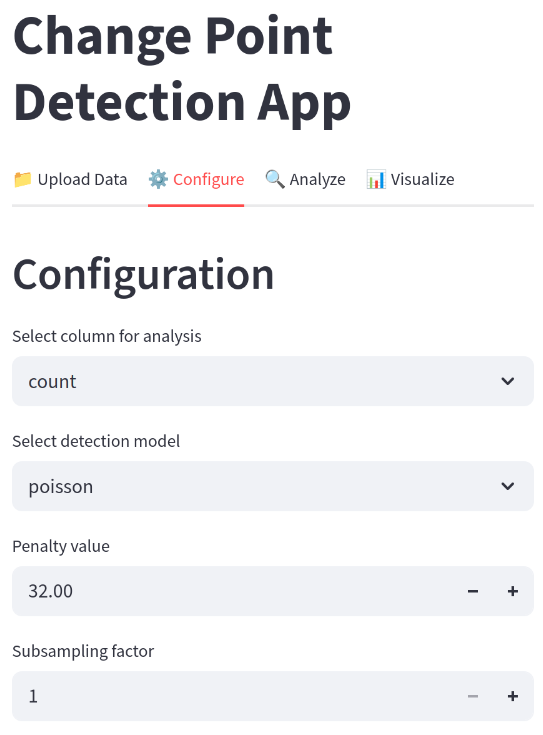
\includegraphics[width=\textwidth]{figures/changepoints-settings.png}
        \caption{Web app: settings}
        \label{fig:changepoints-settings}
    \end{subfigure}
    \hfill
    \begin{subfigure}{0.65\textwidth}
        \centering
        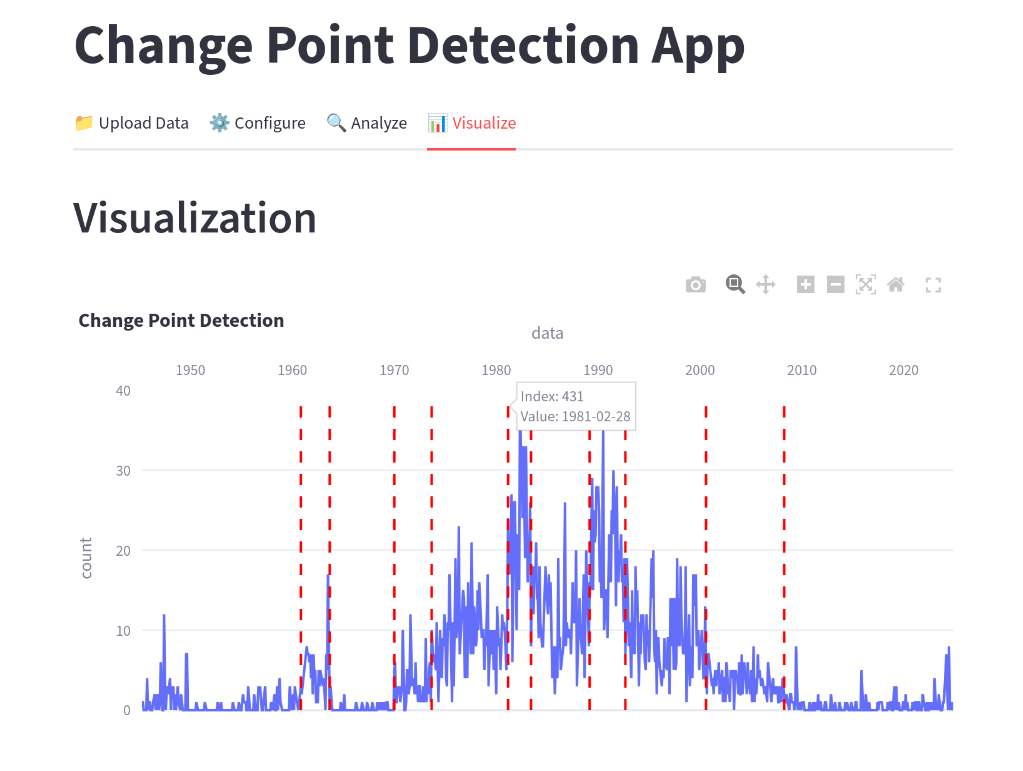
\includegraphics[width=\textwidth]{figures/changepoints.png}
        \caption{Web app: changepoint view}
        \label{fig:changepoints-webapp}
    \end{subfigure}
    \caption{
        Screenshots of the web application developed to visualize and explore the changepoint detection results. From the settings panel (\subref{fig:changepoints-settings}) it's possible to configure the algorithm parameters; the main view (\subref{fig:changepoints-webapp}) shows the time series of murders with detected changepoints in red dashed lines.
    }
    \label{fig:changepoints-webapp-full}
\end{figure}
\section{Attended conferences and publications}

During this year I attended the following conferences:
\begin{itemize}
    \item \textbf{CLS 2025 - Complexity in Living Systems}, Palermo, Italy, July 2025. I helped on the logistics of the event.
    \item \textbf{STATPHYS29}, Florence, Italy, July 2025. I presented a poster named \textit{Mafia Murders as a Complex System: Temporal Patterns and Statistical Modeling}.
    \item \textbf{CCS 25 - Conference on Complex Systems}, Siena, Italy, September 2025. I presented a talk named \textit{Detecting Historical Turning Points in Italian Media: A Complex Systems Approach to a Diachronic News Corpus} at the satellite \textit{COMPLEX R.O.M.E. : COMPLEXity Research On Modeling historical Evolution}.
\end{itemize}

I also worked on the following publications:
\begin{itemize}
    \item G. Glaviano, D. Zarcone, F. Petruzzella, M. Tumminello, S. Miccichè, \textit{Dynamical geolocalization of homicides in the city of Palermo}, in preparation.
    \item D. Zarcone, D. Sanchez, S. Miccichè \textit{Detecting Historical Turning Points in Italian Media: A Complex Systems Approach to a Diachronic News Corpus}, in preparation.
\end{itemize}

\pagebreak

\printbibliography

\end{document}
